\section{Elementary Data Structures}

\begin{description}

\descitem{10.1-1} \textit{Using Figure 10.1 as a model, illustrate the result of each operation in the sequence $\proc{Push}(S,4)$, $\proc{Push}(S,1)$,$\proc{Push}(S,3)$, $\proc{Pop}(S)$, $\proc{Push}(S,8)$, and $\proc{Pop}(S)$  on an initially empty stack $S$ stored in array $S[1 \twodots6]$.}
\begin{ex}
    \begin{figure}[H]
      \centering
      \begin{subfigure}[t]{.45\textwidth}
        \centering
        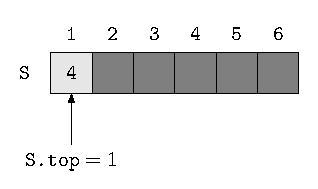
\includegraphics[scale=1]{img/10_1-1/10_1-1_1.pdf}
        \caption{$\proc{Push}(S,4)$}\label{fig:10_1-1_1}
      \end{subfigure}
      \begin{subfigure}[t]{.45\textwidth}
        \centering
        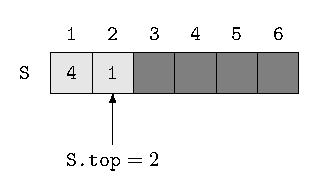
\includegraphics[scale=1]{img/10_1-1/10_1-1_2.pdf}
        \caption{$\proc{Push}(S,1)$}\label{fig:10_1-1_2}
      \end{subfigure}
      \begin{subfigure}[t]{.45\textwidth}
        \centering
        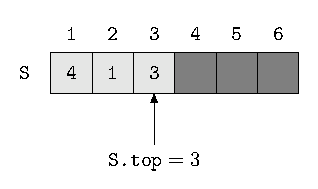
\includegraphics[scale=1]{img/10_1-1/10_1-1_3.pdf}
        \caption{$\proc{Push}(S,3)$}\label{fig:10_1-1_3}
      \end{subfigure}
      \begin{subfigure}[t]{.45\textwidth}
        \centering
        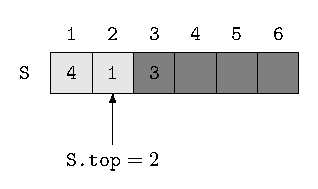
\includegraphics[scale=1]{img/10_1-1/10_1-1_4.pdf}
        \caption{$\proc{Pop}(S)$}\label{fig:10_1-1_4}
      \end{subfigure}
      \begin{subfigure}[t]{.45\textwidth}
        \centering
        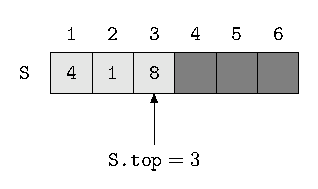
\includegraphics[scale=1]{img/10_1-1/10_1-1_5.pdf}
        \caption{$\proc{Push}(S,8)$}\label{fig:10_1-1_5}
      \end{subfigure}
      \begin{subfigure}[t]{.45\textwidth}
        \centering
        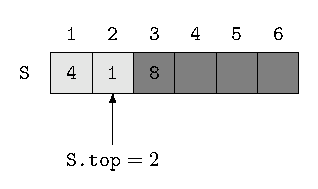
\includegraphics[scale=1]{img/10_1-1/10_1-1_6.pdf}
        \caption{$\proc{Pop}(S)$}\label{fig:10_1-1_6}
      \end{subfigure}
      \caption{Séquence d'opérations sur une pile vide de taille 6.} 
    \end{figure}
\end{ex}
\descitem{10.1-2} \textit{}
\descitem{10.1-3} \textit{}
\descitem{10.1-4} \textit{}
\descitem{10.1-5} \textit{}
\descitem{10.1-6} \textit{}
\descitem{10.1-7} \textit{}


\end{description}
